\documentclass[
  bibliography=totoc,     % Literatur im Inhaltsverzeichnis
  captions=tableheading,  % Tabellenüberschriften
  titlepage=firstiscover, % Titelseite ist Deckblatt
]{scrartcl}
% Paket float verbessern
\usepackage{scrhack}

% Warnung, falls nochmal kompiliert werden muss
\usepackage[aux]{rerunfilecheck}

% unverzichtbare Mathe-Befehle
\usepackage{amsmath}
% viele Mathe-Symbole
\usepackage{amssymb}
% Erweiterungen für amsmath
\usepackage{mathtools}
\usepackage{longtable}

% Fonteinstellungen
\usepackage{fontspec}
% Latin Modern Fonts werden automatisch geladen
% Alternativ:
%\setromanfont{Libertinus Serif}
%\setsansfont{Libertinus Sans}
%\setmonofont{Libertinus Mono}
\recalctypearea % Wenn man andere Schriftarten gesetzt hat,
% sollte man das Seiten-Layout neu berechnen lassen

% deutsche Spracheinstellungen
\usepackage{polyglossia}
\setmainlanguage{german}


\usepackage[
  math-style=ISO,    % ┐
  bold-style=ISO,    % │
  sans-style=italic, % │ ISO-Standard folgen
  nabla=upright,     % │
  partial=upright,   % ┘
  warnings-off={           % ┐
    mathtools-colon,       % │ unnötige Warnungen ausschalten
    mathtools-overbracket, % │
  },                       % ┘
]{unicode-math}

% traditionelle Fonts für Mathematik
\setmathfont{Latin Modern Math}
% Alternativ:
%\setmathfont{Libertinus Math}

\setmathfont{XITS Math}[range={scr, bfscr}]
\setmathfont{XITS Math}[range={cal, bfcal}, StylisticSet=1]

% Zahlen und Einheiten
\usepackage[
  locale=DE,                   % deutsche Einstellungen
  separate-uncertainty=true,   % immer Fehler mit \pm
  per-mode=symbol-or-fraction, % / in inline math, fraction in display math
]{siunitx}

% chemische Formeln
\usepackage[
  version=4,
  math-greek=default, % ┐ mit unicode-math zusammenarbeiten
  text-greek=default, % ┘
]{mhchem}

% richtige Anführungszeichen
\usepackage[autostyle]{csquotes}

% schöne Brüche im Text
\usepackage{xfrac}

% Standardplatzierung für Floats einstellen
\usepackage{float}
\floatplacement{figure}{htbp}
\floatplacement{table}{htbp}

% Floats innerhalb einer Section halten
\usepackage[
  section, % Floats innerhalb der Section halten
  below,   % unterhalb der Section aber auf der selben Seite ist ok
]{placeins}

% Seite drehen für breite Tabellen: landscape Umgebung
\usepackage{pdflscape}

% Captions schöner machen.
\usepackage[
  labelfont=bf,        % Tabelle x: Abbildung y: ist jetzt fett
  font=small,          % Schrift etwas kleiner als Dokument
  width=0.9\textwidth, % maximale Breite einer Caption schmaler
]{caption}
% subfigure, subtable, subref
\usepackage{subcaption}

% Grafiken können eingebunden werden
\usepackage{graphicx}
\usepackage{wrapfig}
% größere Variation von Dateinamen möglich
\usepackage{grffile}

% schöne Tabellen
\usepackage{booktabs}

% Verbesserungen am Schriftbild
\usepackage{microtype}

% Literaturverzeichnis
\usepackage[
  backend=biber,
  urldate=iso8601,
  date=iso8601,
  style=chem-rsc,
  articletitle=true,
]{biblatex}
% Quellendatenbank
\addbibresource{lit.bib}
% Hyperlinks im Dokument
\usepackage[
  unicode,        % Unicode in PDF-Attributen erlauben
  pdfusetitle,    % Titel, Autoren und Datum als PDF-Attribute
  pdfcreator={},  % ┐ PDF-Attribute säubern
  pdfproducer={}, % ┘
]{hyperref}
% erweiterte Bookmarks im PDF
\usepackage{bookmark}

\usepackage{tikz}
\usepackage{tikz-feynman}

% Trennung von Wörtern mit Strichen
\usepackage[shortcuts]{extdash}

\author{%
  Nicole Schulte%
  \texorpdfstring{%
    \\%
    \href{mailto:nicole.schulte@udo.edu}{nicole.schulte@udo.edu}
  }{}%
  \texorpdfstring{\and}{, }%
  Hendrik Bökenkamp%
  \texorpdfstring{%
    \\%
    \href{mailto:hendrik.boekenkamp@udo.edu}{hendrik.bökenkamp@udo.edu}
  }{}%
}
\publishers{TU Dortmund – Fakultät Physik}
\setlength\parindent{0pt}


\subject{V16}
\title{Rutherford-Streuung}
\date{
  Durchführung: 10.01.2018
  \hspace{3em}
  %Abgabe: 25.11.2017
}

\begin{document}

\maketitle
\thispagestyle{empty}
\tableofcontents
\newpage

\section{Ziel}
Es soll der Interferenzkontrast eines Sagnac-Interferometers ermittelt werden.
Außerdem soll mit Hilfe des Sagnac-Interferometers der Brechungsindex von Glas
bzw. Luft ermitelt werden.

\section{Theorie}
\subsection{Sagnac-Interferometer}
\label{sec:SI}

In Abbildung \ref{fig:sagnac} wird der Versuchsaufbau des Sagnac-Interferometers
dargestellt.

\begin{figure}[H]
  \centering
  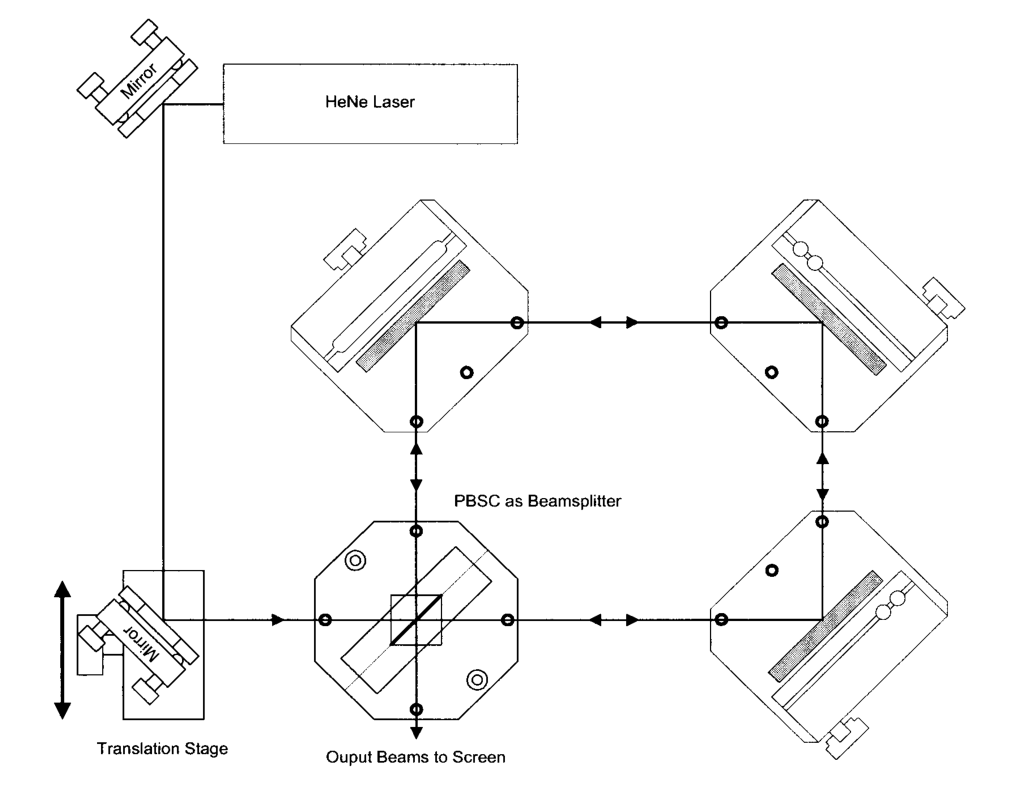
\includegraphics
  [width=12cm]{sagnac.png}
  \caption{Versuchsaufbau des Sagnac-Interferometers. \cite{skript}}
  \label{fig:sagnac}
\end{figure}

Es wird ein HeNe-Laser verwendet, welcher an zwei Spiegeln reflektiert wird und
über ein PBSC (Polarizing Beam-Splitter Cube) in zwei Teilstrahlen aufgeteilt wird.
Die Laserstrahlen werden in entgegengesetzter Richtung an drei Spiegeln im Rechteck
reflektiert und treffen wieder auf den PBSC.
Beide Strahlen legen einen näherungsweise gleichen Weg zurück.
Dort laufen die Teilstrahlen wieder zusammen, welche miteinander interferieren sollen.

Da die zusammenlaufenden Laserstrahlen genau senkrecht aufeinander linear polarisiert
sind, können keine Interferenzen stattfinden.
Daher muss der Strahl erneut in seine Komponenten aufgeteilt werden, um diesen
auszuwerten.
Hierzu wird, wie in Abbildung \ref{fig:separator} dargestellt, ein PBSC verwendet, der um einen 45° Winkel gekippt ist.
Die beiden Teilstrahlen treffen auf jeweils eine Diode.
Die Intensitäten werden als Spannungen auf einem Oszilloskop dargestellt und interpretiert.

\begin{figure}[H]
  \centering
  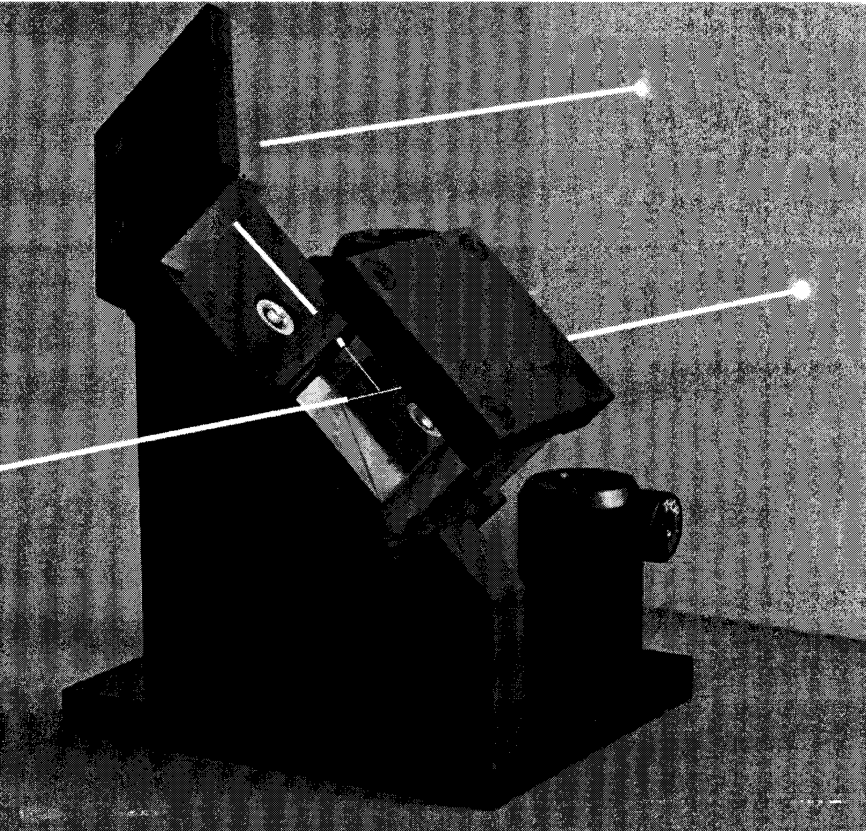
\includegraphics
  [width=10cm]{separator.png}
  \caption{Nutzung des PBSC als Polarisationstrenner. \cite{skript}}
  \label{fig:separator}
\end{figure}

\subsection{Der Interferenzkontrast und Lichtintensität}

Der Interferenzkontrast ist abhängig von der Lichtintensität je nach Polarisationsrichtung.
Der Kontrast ist definiert als
\begin{equation}
  K := \frac{I_{max} - I_{min}}{I_{max} + I_{min}}.
  \label{eqn:kontrast}
\end{equation}
Bei Unkenntlichkeit beträgt dieser Null ($I_{max} = I_{min}$) und im Idealfall gilt $K=1$.

Für die Anteile des Strahls gilt
\begin{gather*}
  E_1 = E_0\cos(\phi)\cos(\omega t) \\
  E_2 = E_0\sin(\phi)\cos(\omega t + \delta),
\end{gather*}
wobei $\delta$ die relative Phasenverschiebung der Teilwellen zueinander beschreibt.
Für die Intensität der überlagerten Strahlen gilt
\begin{equation*}
  I \propto <|E_1 + E_2|>.
\end{equation*}
Durch Einsetzen und durch ausnutzen der Relationen
\begin{gather*}
  <\cos^2(\alpha x + y)> = \frac{1}{2} \\
  \delta = 2\pi n , \, n\in\mathrm{N}_0,\, \text{für konstriktive Interferenz und} \\
  \delta = (2n+2)\pi,\, n\in\mathrm{N}_0,\, \text{für destruktive Interferenz}
\end{gather*}
folgt nach Umformung für konstruktive bzw. destruktive Interferenz
\begin{equation*}
  I_{max/min} \propto \frac{1}{2}E_0^2 (1 \pm 2\cos(\phi)\sin(\phi))
\end{equation*}
bzw.
\begin{equation}
  I_{max/min} \propto I_0(1 \pm 2\cos(\phi)\sin(\phi)).
\end{equation}
Es ergibt sich, dass
\begin{align*}
  K \propto |2\cos(\phi)\sin(\phi)| = |\sin(2\phi)|.
\end{align*}

\subsection{Brechungsindizes}
Allgemein ist der Brechungsindex definiert als
\begin{equation*}
  n = \frac{c}{v},
\end{equation*}
wobei $c$ die Vakuumlichtgeschwindigkeit und $v$ die Phasengeschwindigkeit des Lichts im Medium ist.
Bei gutem Kontrast kann die Anzahl der Maxima durch die Phasenverschiebung eines
der Strahlen abgezählt werden. Die Phasenverschiebung kann durch eine Gaszelle,
in der der Druck kontinuierlich verändert werden kann, oder durch einen rotierbaren
transparenten Festkörper erzeugt werden.
Allgemein gilt für die Anzahl der Maxima
\begin{equation*}
  M = \frac{\delta}{2\pi},
\end{equation*}
wobei $\delta$ die Phasenverschiebung eines gestörten Strahls gegenüber eines
ungestörten Lichtstrahls angibt.
Der Brechungsindex $n$ von Luft in einer Gaszelle lässt sich mittels der Formel
\begin{equation}
  %n(p_0, T_0) = 1 + \Delta n(p_1,p_2)\frac{T}{T_0}\frac{p_0}{p_2-p_1}
  M = \frac{n-1}{\lambda_{\text{vac}}}\cdot{L}
  \label{eqn:brechluft}
\end{equation}
berechnen,
%wobei $p_0 = 1013,2$mbar und $T_0 = 273,15$K die Standardbedingungen darstellen.
wobei $M$ die Anzahl der Maxima, $\lambda$ die Wellenlänge und $L$ die Länge der Gaszelle ist.

Für den Brechungsindex eines Festkörpers wird eine Halterung für zwei Glasplatten,
die in einem Winkel von $\alpha = 2\cdot\theta_0 = 20°$ zueinander stehen, verwendet.
Allgemein ist Eine Funktion für die Anzahl der Maxima durch eine Glasplatte gegeben durch
\begin{equation}
  M = \frac{T}{\lambda}\cdot\frac{n-1}{2n}\cdot\theta^2.
\label{M_allg}
\end{equation}
Dabei ist $T$ die Dicke der Glasplatte, $\lambda$ die Wellenlänge des Lichts, $n$ der Brechungsindex des Materials und $\theta$ der Rotationswinkel.
Da in diesem Versuch aber zwei Glasscheiben, die in einem relativen Winkel zueinander stehen, verwendet werden,
muss die Formel \eqref{M_allg} über die beiden Winkel $\theta = \theta_0$ und $\theta = -\theta_0$ Taylor-entwickelt werden.
Es ergeben sich
\begin{gather*}
  (\mathcal{T}M)^{(1)}(\theta,\theta_0) = \frac{T}{\lambda}\cdot\frac{n-1}{2n}(\theta^2 + 2\theta_0(\theta-\theta_0)),\\
  (\mathcal{T}M)^{(1)}(\theta,-\theta_0) = \frac{T}{\lambda}\cdot\frac{n-1}{2n}(\theta^2 - 2\theta_0(\theta+\theta_0)).
\end{gather*}
Die Differenz der beiden Entwicklungen liefert
\begin{equation*}
  M_{\mathcal{T}}(\theta) :=
  (\mathcal{T}M)^{(1)}(\theta,\theta_0) - (\mathcal{T}M)^{(1)}(\theta;-\theta_0)
   = \frac{T}{\lambda}\cdot\frac{n-1}{2n}\cdot(4\theta_0\theta)
 \end{equation*}
 Umgestellt nach dem Brechungsindex ergibt sich die Formel,
 mit der sich der Brechungsindex des transparenten Festkörpers berechnen lässt:
\begin{equation}
  n = \left( 1 - \frac{\lambda{M}}{2T\theta_0\theta} \right)^{-1}
  % = \frac{-2 \theta_0\theta T}{M\lambda - 2 T\theta\theta_0}.
\label{eqn:glas}
\end{equation}
Hierbei ist $M = M_{\mathcal{T}}(\theta)$.

\section{Durchführung}

In dem Experiment wird der in Abbildung \ref{fig:aufbau} dargestellte Aufbau
verwendet.

\begin{figure}[H]
  \centering
  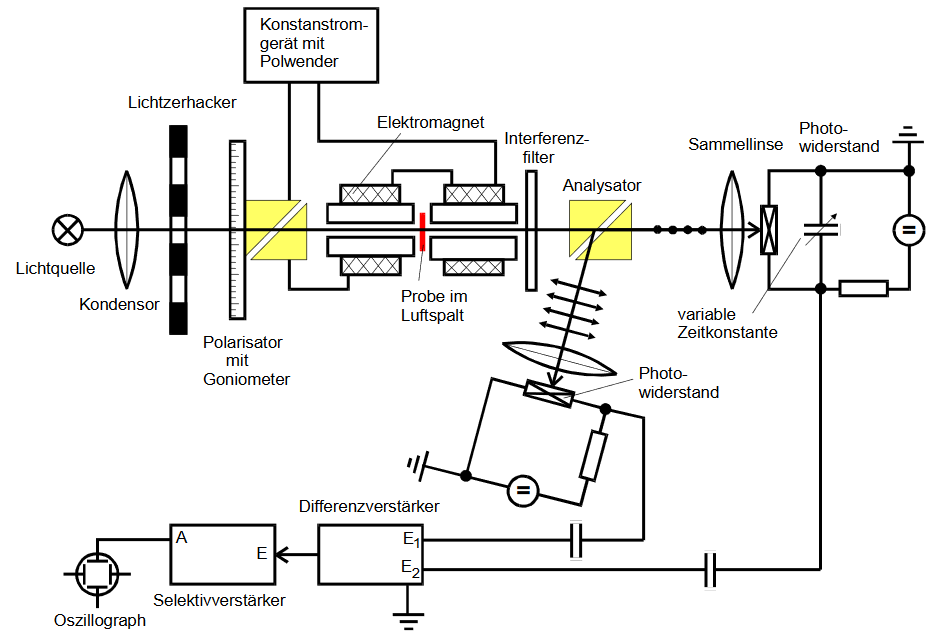
\includegraphics[width=8cm]{aufbau.png}
  \caption{In dem experiment verwendeter Aufbau}
  \label{fig:aufbau}
\end{figure}

Zu Beginn der Messung wird der Rezipient evakuiert und dann mit Helium gefüllt.
Das Dewar-Gefäß, das den Rezipienten umgibt, wird dann mit flüssigem
Stickstoff gefüllt, damit der Rezipient die Temperatur von dem Stickstoff, also
ungefähr $\SI{80}{\kelvin}$ annimmt. Der Vorgang der Temperaturübertragung
dauert ungefähr $\SI{1}{\hour}$. Danach wird der Rezipient erneut evakuiiert,
um Wärmeverlust durch Konvektion zu vermeiden. Die kalte Probe im Rezipienten
wird dann mit Hilfe einer Heizwicklung erwärmt, ihr wird also elektrische
Energie zugeführt. Zur Messung der Temperatur wird ein Thermoelement verwendet,
welches einen Widerstand misst.

Energieverluste können in diesem Versuch nicht nur durch Konvektion, also
den Wärmeverlust durch Teilchenströme, entstehen. Ein weiterer Energieverlust
ist durch Wärmestrahlung gegeben. Wird die Probe erhitzt, so gibt strahlt sie
Wärme ab. Um diese Verluste zu minimieren, wird um die Probe ein Gehäuse
gestellt, welches auf die Temperatur der Probe geregelt wird. Dadurch strahlt
auch dieses Gehäuse Wärme ab, welches von der Probe wieder aufgeommen wird.
Dadurch sollte bei optimaler Abstimmung der Wärmeverlust durch Wärmestrahlung
verringert werden. Zudem kann Energie durch Wärmeleitung an die Bauteile
verloren gehen.

\section{Bestimmung des Bremsvermögens von Alphateilchen in Luft}
Die Reichweite von Luft kann mit der Formel \eqref{eqn:bloch} bestimmt werden.
Im Folgenden wird angenommen, dass die Luft aus $80\,\%$ Stickstoff und $20\,\%$ Sauerstoff besteht.
Die Geschwindigkeit des $\alpha$-Teilchens beträgt $v_{\alpha}= 1,625\cdot10^{7}\,\frac{\text{m}}{\text{s}}$ (siehe Abschnitt \ref{gofodi}).
Die Teilchendichte lässt sich über den Zusammenhang
\begin{align*}
  n = \rho/m
\end{align*}
berechnen.
Dabei ist die Luftdichte $\rho_{\text{Luft}} = 1,204\,\frac{\text{kg}}{\text{m}^3}$ \cite{chem2} und die gemittelte Masse
$m = 14,4 \,\text{u}$ \cite{PSE}.
Damit ist die Teilchendichte von Luft $n_{\text{Luft}} = 5,04\cdot10^{25}\,\text{m}^{-3}$.
Die mittlere Ionisierungsenergie von Luft ist
$\overline{I}_{\text{Luft}} = 14,32\,\text{eV}$ \cite{PSE}.
Die Kernladungszahl der $\alpha$-Teilchen ist $z=2$ und die effektive Kernladungszahl von Luft beträgt
$Z_{\text{eff}} = 7,2$.
Mit diesen Daten lässt sich das Bremsvermögen berechnen. Dieses beträgt
\begin{equation*}
  -\frac{dE}{dx} = 134,66\,\frac{\text{keV}}{\text{mm}}
\end{equation*}
Wird das ideale Gasgesetz
\begin{equation}
  n = \frac{N}{V} = \frac{p}{k_{\text{B}}T}
\end{equation}
in Formel \eqref{eqn:bloch} eingesetzt,
ist ein linearer Zusammenhang zu erkennen.
Unter Berücksichtigung von Standardbedingungen ($T= 298,15\,\text{K}$), kann darüber die Druckabhängigkeit des Energieverlustes bestimmt werden.
Sobald sich die Energie des $\alpha$-Teilchens in $10^{-2}\,\text{m}$ um $5\,\%$ verringert, macht sich der Energieverlust bemerkbar.
Das heißt, dass
\begin{align*}
  -\frac{dE}{dx} = 0,05\cdot\frac{E_{\alpha}}{1\,\text{mm}}.
\end{align*}
Der Wert von $E_{\alpha}$ kann dem Abschnitt \ref{gofodi} entnommen werden.
Durch Umstellen nach $p$ kann der Druck, bei dem sich Energieverluste bemerkbar machen, berechnet werden.
Dieser beträgt
\begin{align*}
  p = 0,4\,\text{bar}.
\end{align*}

\section{Auswertung}
\subsection{Kontrastmessung}
Zunächst muss für eine bessere Qualität der späteren Messung der Kontrast
ermittelt werden. Mit Hilfe von Formel \eqref{eqn:kontrast} wird dieser
berechnet. Die gemessenen Spannungen mit den zugehörigen Winkeln werden in
Tabelle \ref{tab:kontrast} dargestellt.

\begin{table}
[H]
  \centering
\begin{tabular}{cccc}

  \toprule
$\phi \ [\si{\degree}]$ & $U_\text{min} \ [\SI{}{\volt}]$ &
$U_\text{max} \ [\SI{}{\volt}]$ & $K$ \\
\midrule

195 & \SI{1.28}{} & \SI{2.70}{} & \SI{0.36}{} \\

180 & \SI{1.52}{} & \SI{1.82}{} & \SI{0.09}{} \\

165 & \SI{0.76}{} & \SI{2.01}{} & \SI{0.45}{} \\

150 & \SI{0.24}{} & \SI{1.70}{} & \SI{0.75}{} \\

135 & \SI{0.06}{} & \SI{1.30}{} & \SI{0.91}{} \\

120 & \SI{0.10}{} & \SI{0.95}{} & \SI{0.81}{} \\

105 & \SI{0.26}{} & \SI{0.82}{} & \SI{0.52}{} \\

90  & \SI{0.67}{} & \SI{0.81}{} & \SI{0.09}{} \\

75  & \SI{0.47}{} & \SI{1.57}{} & \SI{0.54}{} \\

60  & \SI{0.15}{} & \SI{2.66}{} & \SI{0.89}{} \\

45  & \SI{0.14}{} & \SI{3.41}{} & \SI{0.92}{} \\

30  & \SI{0.54}{} & \SI{3.13}{} & \SI{0.71}{} \\

15  & \SI{1.21}{} & \SI{2.75}{} & \SI{0.39}{} \\

0   & \SI{1.64}{} & \SI{1.90}{} & \SI{0.07}{} \\

-15 & \SI{0.70}{} & \SI{2.00}{} & \SI{0.48}{} \\

\bottomrule
\end{tabular}

\caption{Berechneter Kontrast in Abhängigkeit der Polarisationsrichtung}
\label{tab:kontrast}
\end{table}



Die Ausgleichsfunktion lautet
\begin{equation}
  f(\phi) = a \cdot \lvert \sin(b \cdot \phi +c) \rvert +d
\end{equation}
Die Messwerte und die Ausgleichsfunktion sind in Abbildung \ref{fig:kontrast}
dargestellt.

Für die Parameter ergeben sich die folgenden Werte
\begin{align*}
  a &= \SI{0.88 \pm 0.05}{} \\
  b &= \SI{2.00 \pm 0.02}{\per\radian} \\
    &\hat{=}\, \SI{114.82 \pm 1.03}{\per\degree} \\
  c &= \SI{-0.06 \pm 0.04}{} \\
  d &= \SI{0.03 \pm 0.03}{} \\
\end{align*}

Der Parameter $a$ beschreibt die Amplitude, $b$ eine Frequenz, $c$ die
Phasenverschiebung und $d$ den Kontrastoffset.
Zur Berechnung des optimalen Polarisationswinkel wird das Maximum der
Ausgleichsfunktion ermittelt.
\begin{equation}
  \phi = \frac{1}{b} \left(\frac{\pi}{2} -c \right)
\end{equation}
Dadurch ergibt sich ein Winkel von
\begin{align*}
  \phi &= \SI{0.82 \pm 0.02}{\radian} \\
       &\hat{=} \, \SI{46.72 \pm 1.26}{\degree} \\
\end{align*}
Der Fehler berechnet sich mit Hilfe der Gaußschen Fehlerfortpflanzung
\begin{equation}
  \Delta \phi =\sqrt{\left(- \frac{1}{b^2} \left(\frac{\pi}{2} -c \right)  \right)^2
  \Delta b^2 + \left(- \frac{1}{b}\right)^2 \Delta c^2}
\end{equation}

\begin{figure}[H]
  \centering
  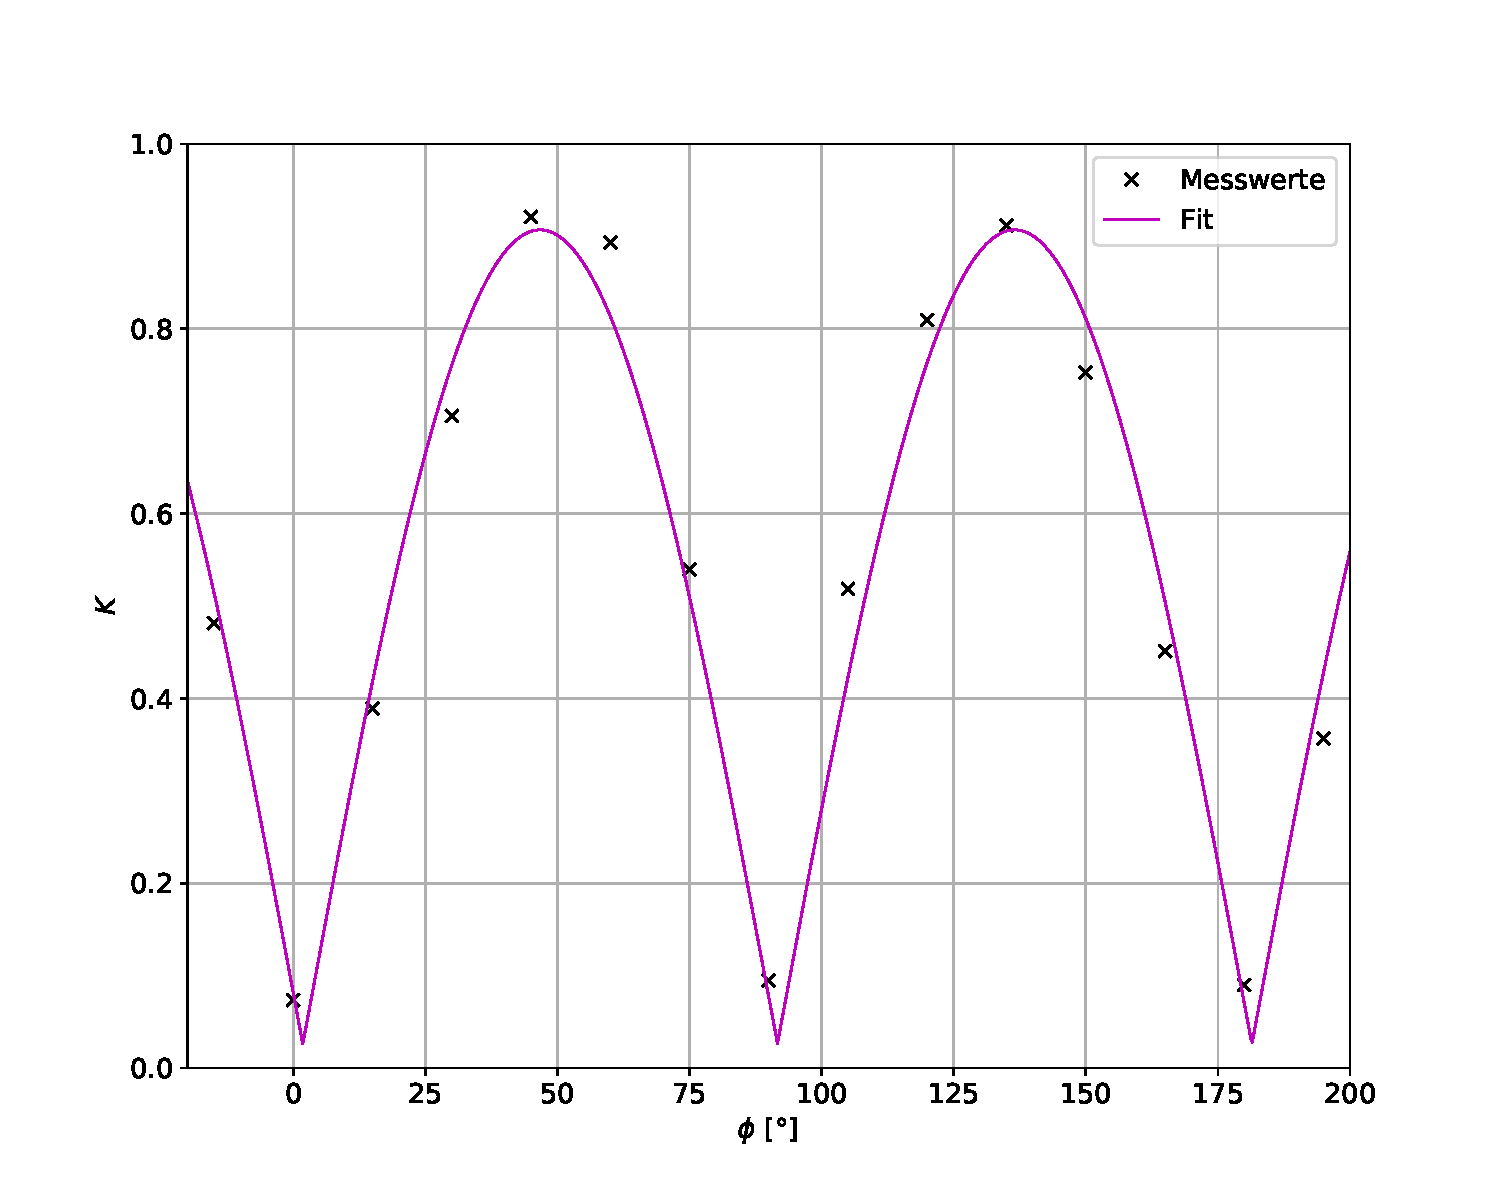
\includegraphics[width=\textwidth]{kontrast.pdf}
  \caption{Kontrast in Abhängigkeit der Polarisationsrichtung mit
  Ausgleichsrechnung}
  \label{fig:kontrast}
\end{figure}
\subsection{Berechnung des Brechungsindex von Glas}
Die gemessenen Maxima mit den zugehörigen Winkeländerungen sind in Tabelle
\ref{tab:glas} dargestellt. Der Brechungsindex berechnet sich mit Hilfe
der Formel \ref{eqn:glas}. Die zugehörigen Brechungsindizes sind neben den
Wertepaaren aufgelistet.

\begin{table}
  \centering
\begin{tabular}{SSSSSSSSS}
  \toprule
  \multicolumn{3}{c}{Messung 1} &\multicolumn{3}{c}{Messung 2}
  & \multicolumn{3}{c}{Messung3} \\
$\phi \, [\si{\radian}]$ & $M$ & $n$ & $\phi \, [\si{\radian}]$ & $M$ & $n$ &
 $\phi \, [\si{\radian}]$ & $M$ & $n$\\
2 & 6 & 1.451 & 2 & 6 & 1.451 & 2 & 5 & 1.35 \\

2 & 7 & 1.569 & 2 & 7 & 1.569 & 2 & 6 & 1.451 \\

2 & 8 & 1.708 & 2 & 7 & 1.569 & 2 & 8 & 1.708 \\

2 & 7 & 1.569 & 2 & 6 & 1.451 & 2 & 7 & 1.569 \\

2 & 6 & 1.451 & 2 & 7 & 1.569 & 2 & 6 & 1.451 \\

\bottomrule
\end{tabular}
\caption{Gemessene Anzahl der Maxima pro Winkeländerung}
\label{tab:glas}
\end{table}


Es ergibt sich ein Mittelwert mit der zugehörigen Standardabweichung von
\begin{align*}
  \bar{n} = \SI{1.526 \pm 0.097}{} \, .\\
\end{align*}

Die Herstellerangabe \cite{skript} für den Brechungsindex lautet

\begin{align*}
  n_H = \SI{1.5}{} \, .
\end{align*}

Das entspricht einer prozentualen Abweichung von $\SI{0.017}{\%}$.

\subsection{Berechnung des Brechungsindex von Luft}

Für die Messungen des Brechungsindex von Luft ergeben sich folgende Werte
\begin{align*}
  \text{Messung 1} &= \SI{42}{}\, \text{Counts} \\
  \text{Messung 2} &= \SI{42}{}\, \text{Counts} \\
  \text{Messung 3} &= \SI{42}{}\, \text{Counts} \, . \\
\end{align*}
Es muss beachtet werden, dass kein vollständiges Vakuum erreicht werden konnte
und das der Wert des erreichten Normaldrucks nicht dem üblichen Wert von
$p_a= \SI{1013}{\milli\bar}$ \cite{druck} entspricht. Die erreichten Druckwerte sind in
diesem Versuch die Folgenden.
\begin{align*}
  p_{\text{min}} &= \SI{1002}{\milli\bar} \\
  p_0            &= \SI{5}{\milli\bar} \\
\end{align*}

Zur Berechnung des Brechungsindes von Luft wird Formel \ref{eqn:brechluft}
verwendet. Die Länge der Messzelle $L$ und die Wellenlänge des Lasers
haben dabei die folgenden Werte.

\begin{align*}
  L &= \SI{100 \pm 0.1}{\milli\meter} \\
  \lambda &= \SI{632.990}{\nano\meter} \\
\end{align*}

Dadurch ergeben sich für die einzelnen Messung die folgenden Brechunsindizes.
\begin{align*}
  n_1 &= \SI{1.000266}{} \\
\end{align*}
Wird lediglich der Fehler der Messzelle berücksichtig, so ergibt sich mittels
Gaußscher Fehlerfortpflanzung ein Wert von
\begin{align*}
  n = \SI{1.000266 \pm 0.000006}{} \, .\\
\end{align*}
Dies ist jedoch ein Fehler der nicht der Messung entspricht. Beim Vakuumieren
der Gaszelle ist auf dem Oszilloskop eine Sinusschwingung zu erkennen. Diese
Schwingungen entsprechen dabei den durchlaufenden Interferenzmaxima. Nachdem
die Zelle vollständig vakuumiert wird, ist trotzdem noch eine getreckte
Sinusschwingung zu erkennen. Das Messgerät misst einen Count, wenn die
Sinusschwingung die Nulllinie übertritt und fast ihr Maximum erreicht. Das
Bedeutet, dass es eine Auswirkung auf die Anzahl der Counts hat, wo die
Messung begonnen wird. Das ist eine Fehlerquelle die mit einberechnet werden
muss. Da die Counts nur diskrete Werte annehmen können, wird dem Messwert
der Counts auch ein diskreter Fehler zugeordnet

\begin{align*}
  M &= 41 \pm 1 \, .\\
\end{align*}

Der Fehler berechnet sich dann mit Hilfe der Gaußschen Fehlerfortpflanzung

\begin{align*}
  \Delta{n} = \sqrt{\left( -\frac{M L}{2L} \right)^2 \cdot \Delta{L}^2
  + \left(\frac{\lambda}{2 L} \right)^2 \cdot \Delta{M}^2} \, .
\end{align*}
Dadurch ergibt sich für den Brechungsindex von Luft ein Wert von

\begin{align*}
n &= \SI{1.0001329 \pm 0.0000032}{} \, .
\end{align*}

Der Theoriewert für den Brechungsindex von Luft lautet
\begin{align*}
  n = \SI{1.000272}{} \, .
\end{align*}
Das entspricht einer Abweichung von $\SI{0.014}{\%}$.

\section{Diskussion}

Die Kurve des Magnetfeldes \ref{fig:B(z)} weist einen realistischen Verlauf auf.
Das Maximum kann hier gut abgeschätzt werden. \\

In Abb. \ref{fig:0(y)} sind keine Regelmäßigkeiten der Rotationswinkel in Abhängigkeit der Wellenlägen zu sehen.
Dies ist ein Indiz einer fehlgeschlagenen Messung. \\

In den Abbildungen \ref{fig:winkeldiff1} und \ref{fig:winkeldiff2} sind große Abweichungen vorzuweisen.
Die Abweichungen der Abbildung \ref{fig:winkeldiff1} sind wesentlich größer als die der \ref{fig:winkeldiff2}.
Auch hier wird die Ungenauigkeit der Messung verdeutlicht. \\

Die empirische effektive Masse $m_1^*$ weicht um 89.8\% von der theoretischen effektiven Masse $m_{\Gamma}$ ab.
Die effektive Masse $m_2^*$ weicht um 64.1\% vom Theoriewert ab. \\

Ein Grund für die Abweichungen kann der fast immer nicht mögliche Abgleich der Spannung am Oszilloskop sein.
Meistens musste ein Minimum der Spannung abgeschätzt werden, was aber nicht immer möglich war.
Teilweise hat sich die Spannung garnicht verändert, sodass die Abschätzung des Minimums erschwert wurde.
Eine mögliche Fehlerquelle kann eine fehlgeschlagene Justierung der Apparatur sein.
Durch die Falsche Justierung können äußere Einflüsse, wie Licht etc. für falsche Werte gesorgt haben.
Außerdem gab es bei dem Abgleich jeweils zwei verschiedene Winkel des Goniometers, die eingestellt werden konnten,
die im Oszilloskop ein Minimum aufgewiesen haben. Dadurch wusste man nicht, welcher Winkel der richtige ist.
Dadurch können möglicherweise falsche Differenzen der Formel \eqref{eqn:thetadiff} entstanden sein.



\nocite{*}
\printbibliography

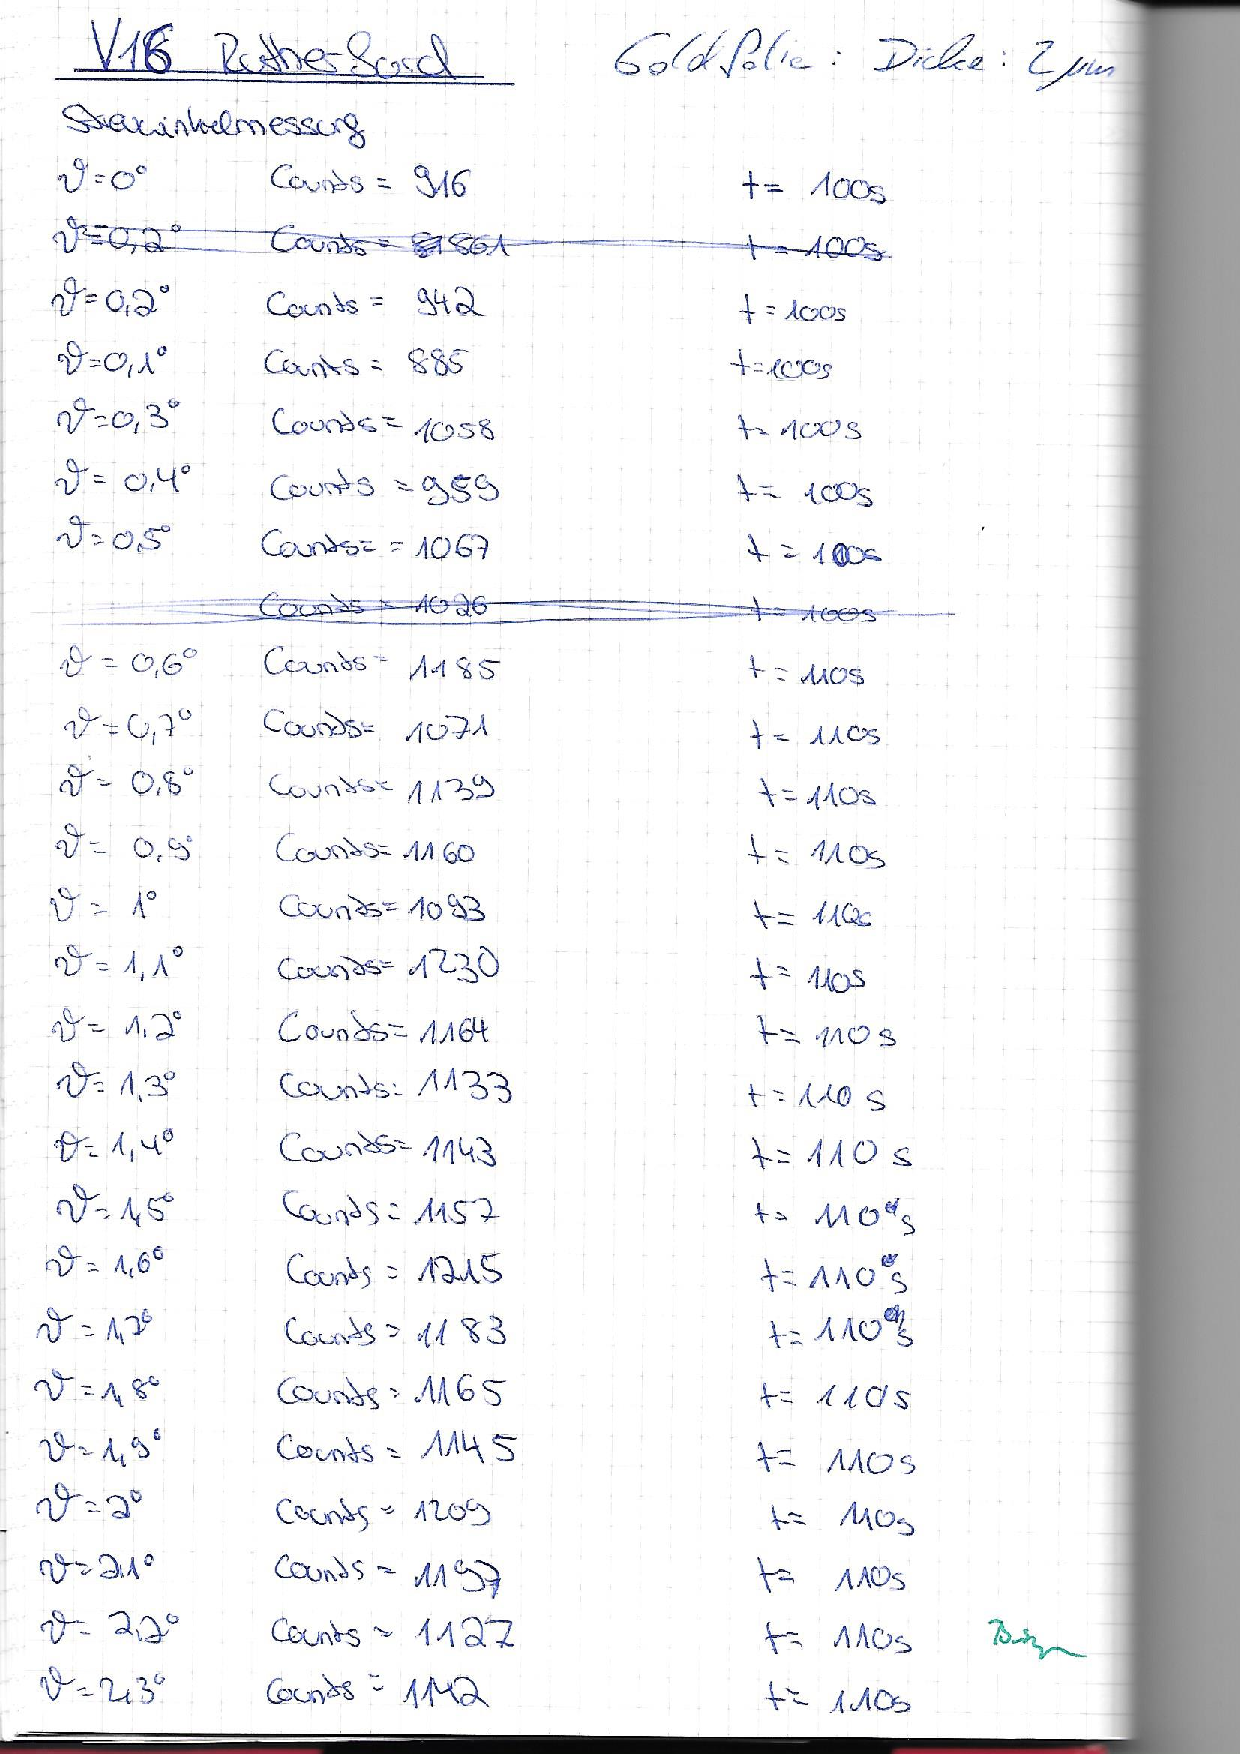
\includepdf[pages=1-]{Scan0001.pdf}
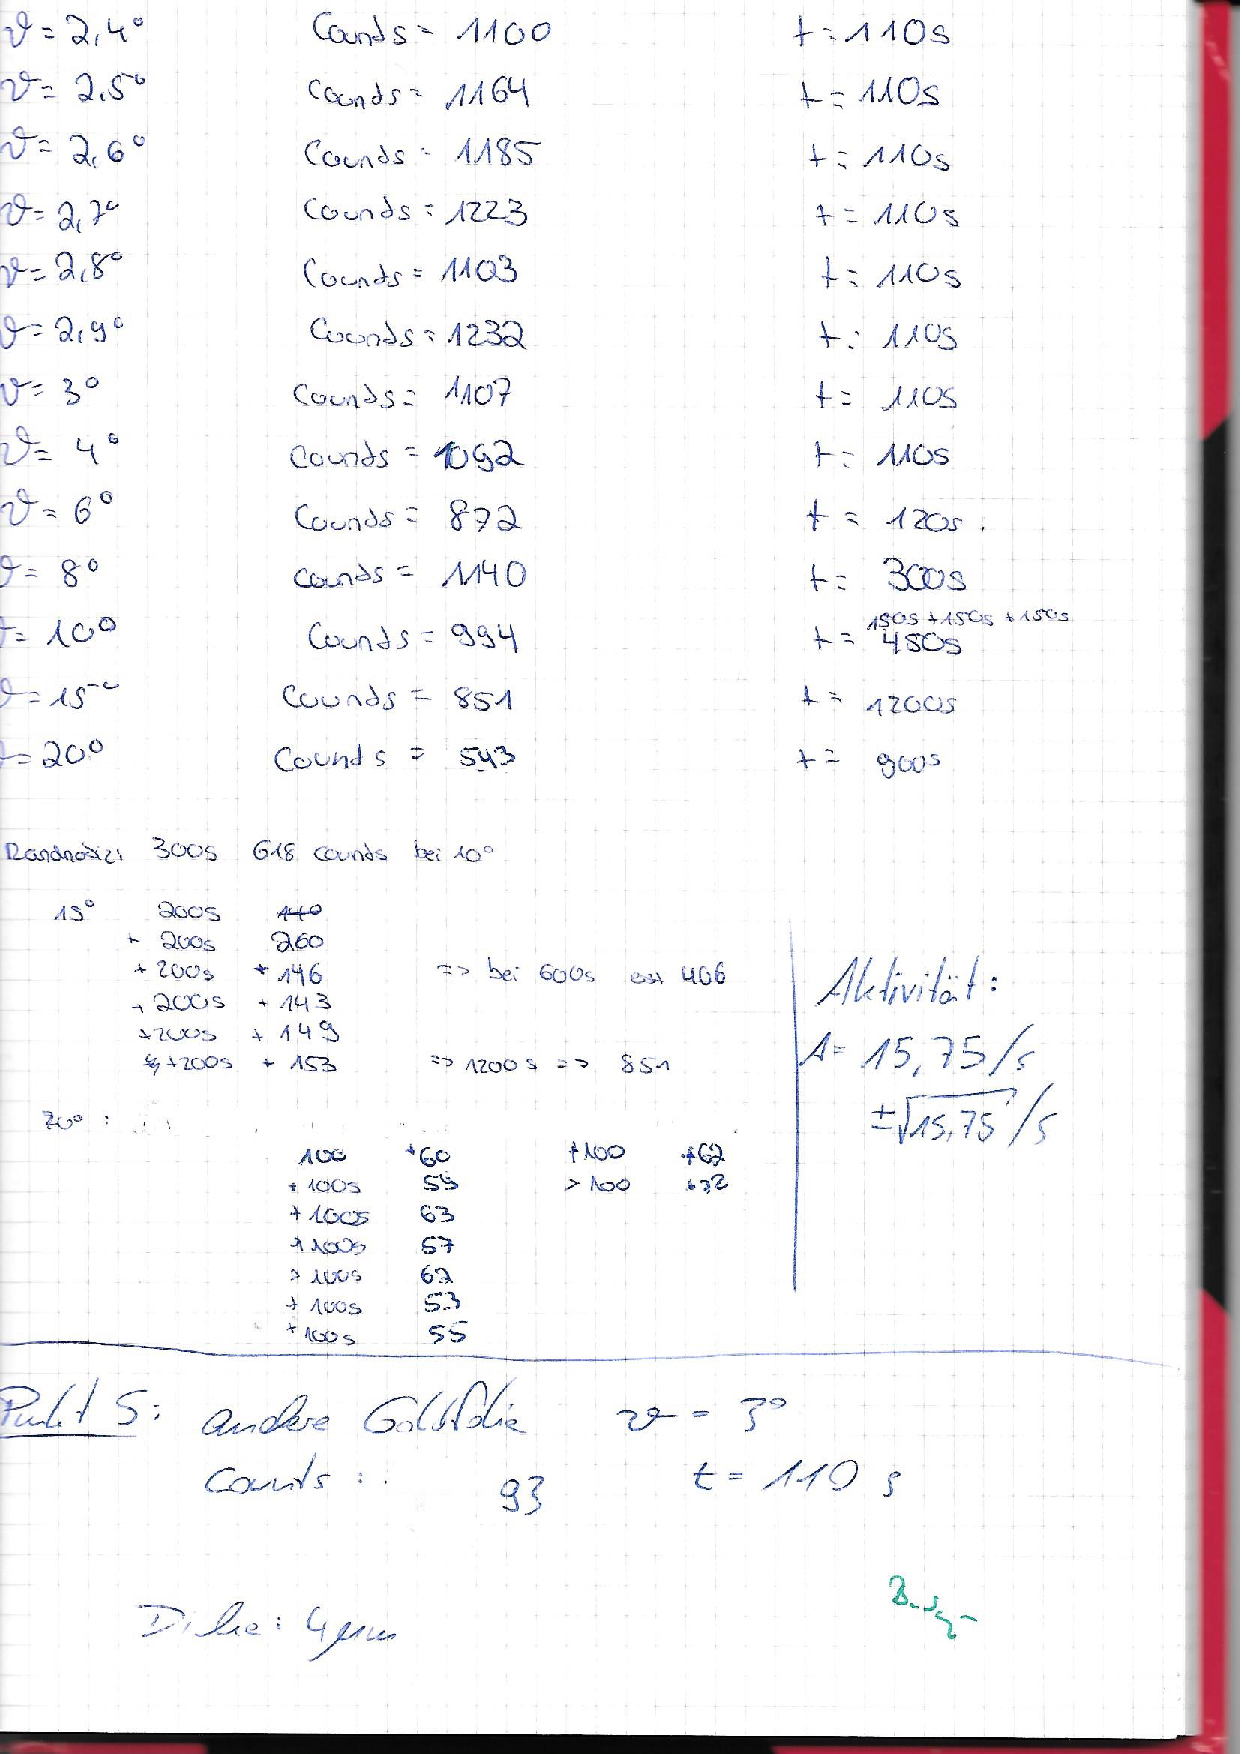
\includepdf[pages=1-]{Scan0002.pdf}
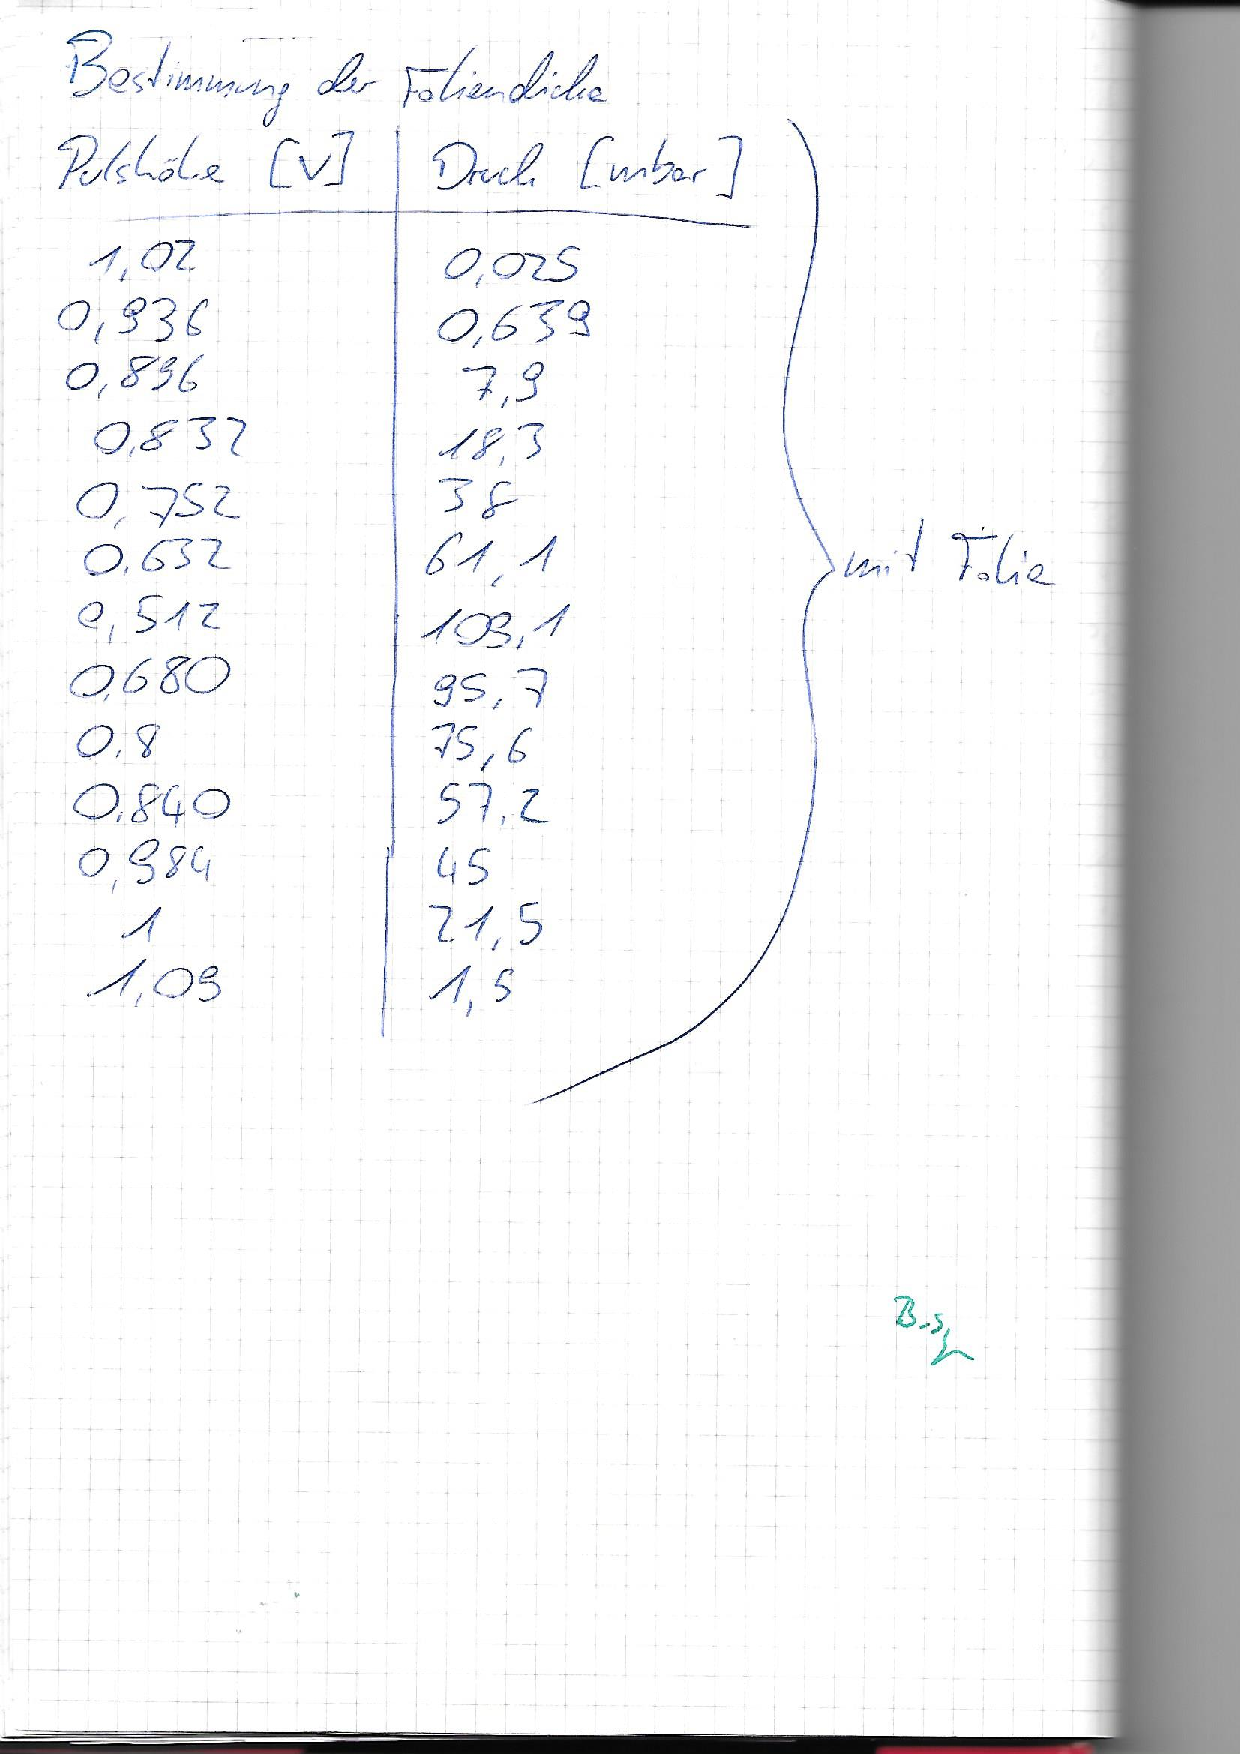
\includepdf[pages=1-]{Scan0003.pdf}
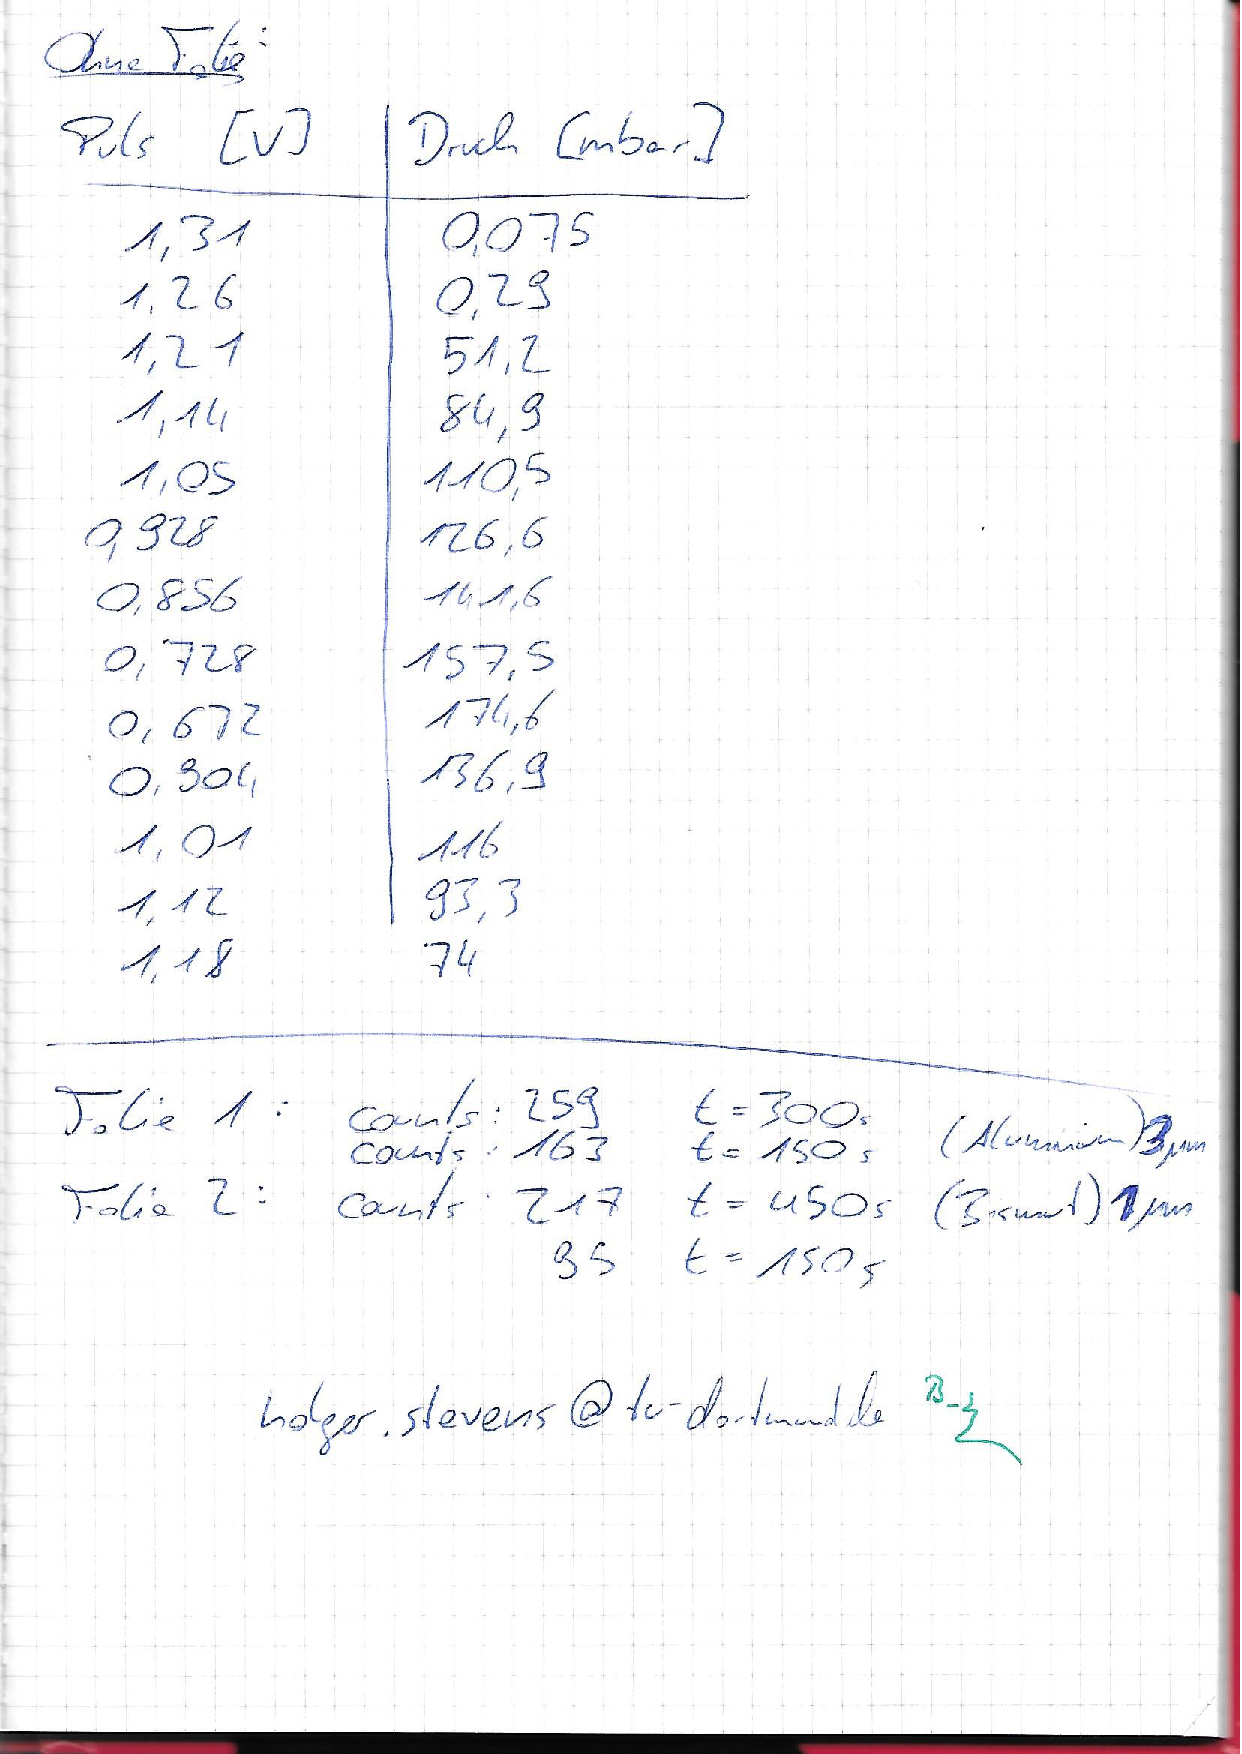
\includepdf[pages=1-]{Scan0004.pdf}
%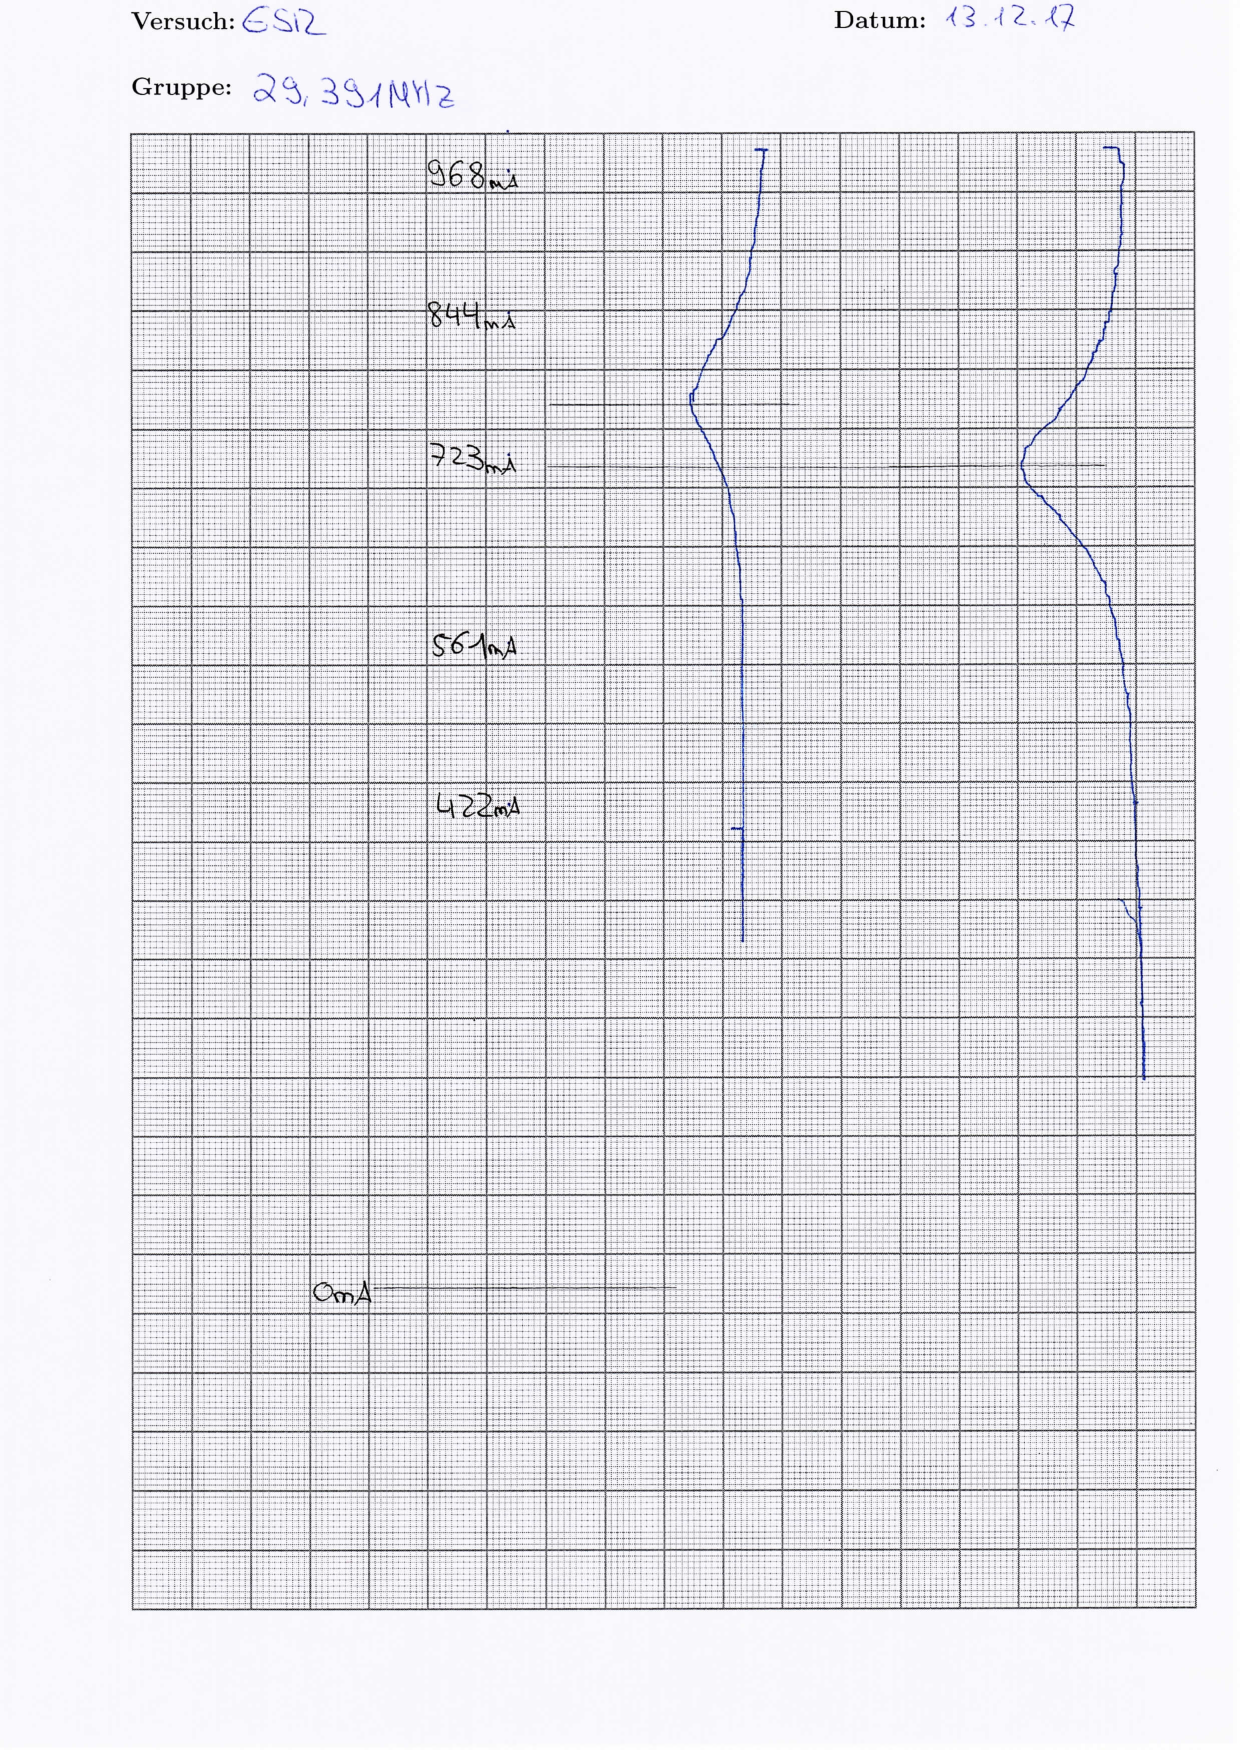
\includepdf[pages=1-]{img005.pdf}

\end{document}
